

\section{National sepsis registry}
The \pmu can act as a leading user for a national sepsis registry.
Our analysis of public and private data allow us to accurately measure the number of cases per year in all institutions.
We can also provide examples of key data that is most valuable including routing clinical and demographic features, examples of how databases are structured, and example of how advance statistical analysis can use this data in daily management and research projects in combination with new technologies. 
Figure 
\ref{fig:national_registry1} (summary) and \ref{fig:national_registry2} (detailed)
 illustrates how we can accurate model the requirements of a national registry database:

\begin{itemize}
\item We can state that the total number of sepsis cases for 2010-2022 was 368'719. A typical year (2022) had 35'205 cases with per-institution averages of 22 (sd: 57, min-max 0-600). The total subset of primary and secondary diagnosis during this period was 245'552.
\item We can give a breakdown of estimated numbers accurate for each institution.
\item We can identify the key players which have the largest number of adult and child cases (e.g. Insel Gruppe, Universitatsspital Zurich, Kantonsspital Baselland).
\item We can reproduce the numbers of main diagnosis per year as reported by FOPH BAG and OBSAN, shown in \textbf{table \ref{tab:year_report}}.
\end{itemize}

\begin{table}[h!]
\centering
\caption{Number of cases in 2022. HD (Hauptdiagnose) und ND (Nebendiagnose), HD and ND are German abbreviations for Principal and Secondary diagnoses, respectively.}
\label{tab:number_of_cases}
\begin{tabular}{lccc}
\hline
\textbf{Diagnosis} & \textbf{Total Number of Cases} & \textbf{Number of Hospitalisations} & \textbf{Average Number of Cases per Hospital} \\
\hline
J.2.1.F HD & 11'782 & 109 & 108 \\
J.2.4.F ND & 5'541 & 103 & 54 \\
\hline
\end{tabular}
    \label{tab:year_report}
\end{table}

\textbf{The database for a Swiss national sepsis registry until spanning from 2010-2030 will contain 400'000 cases. 
For each case it will contain at least a minimal set of 40 demographic and clinical data variables.}
We can advise on the architecture of the database and recommend commercial solutions for hosting a secure and accessible platform.

\begin{figure}[h] \hspace*{0cm} 
\begin{center}
	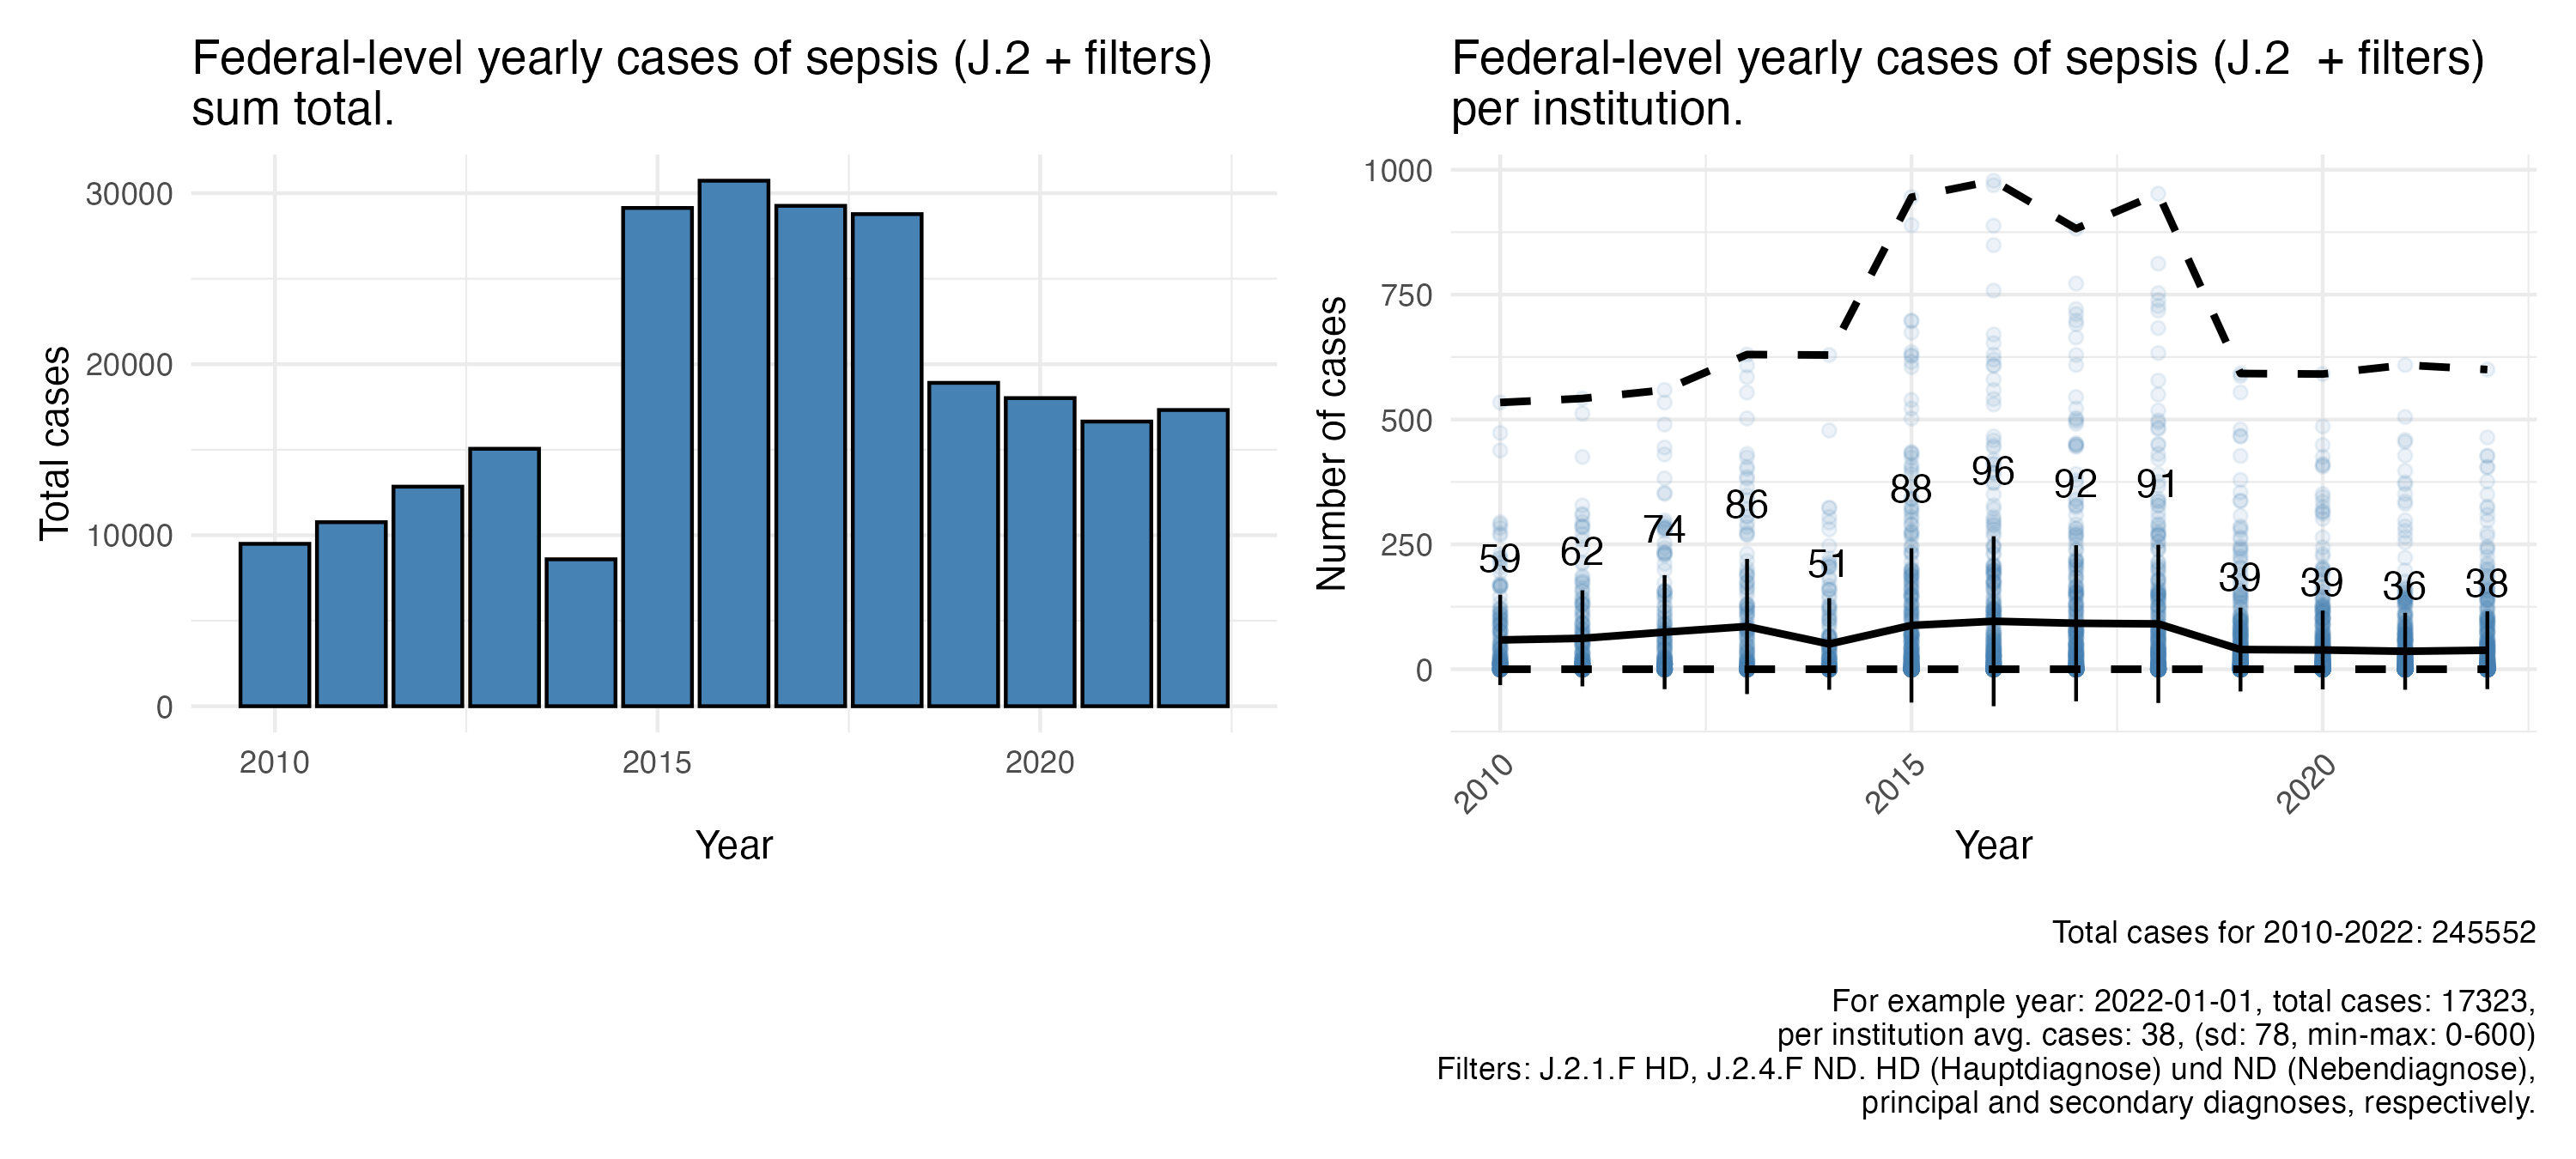
\includegraphics[width=0.90\textwidth]{../stats/foph_key_stats/output/p_patch_tally_main}
	\caption{Cases per year for a national registry (summary). Federal level number of sepsis cases from 2010-2022. These number demonstrate the number of observations required for a national registry. Federal statistics from Bundesamt für Gesundheit (BAG, Federal office for public health).}
	\label{fig:national_registry1}
\end{center}
\end{figure}

\begin{figure}[h] \hspace*{0cm} 
\begin{center}
	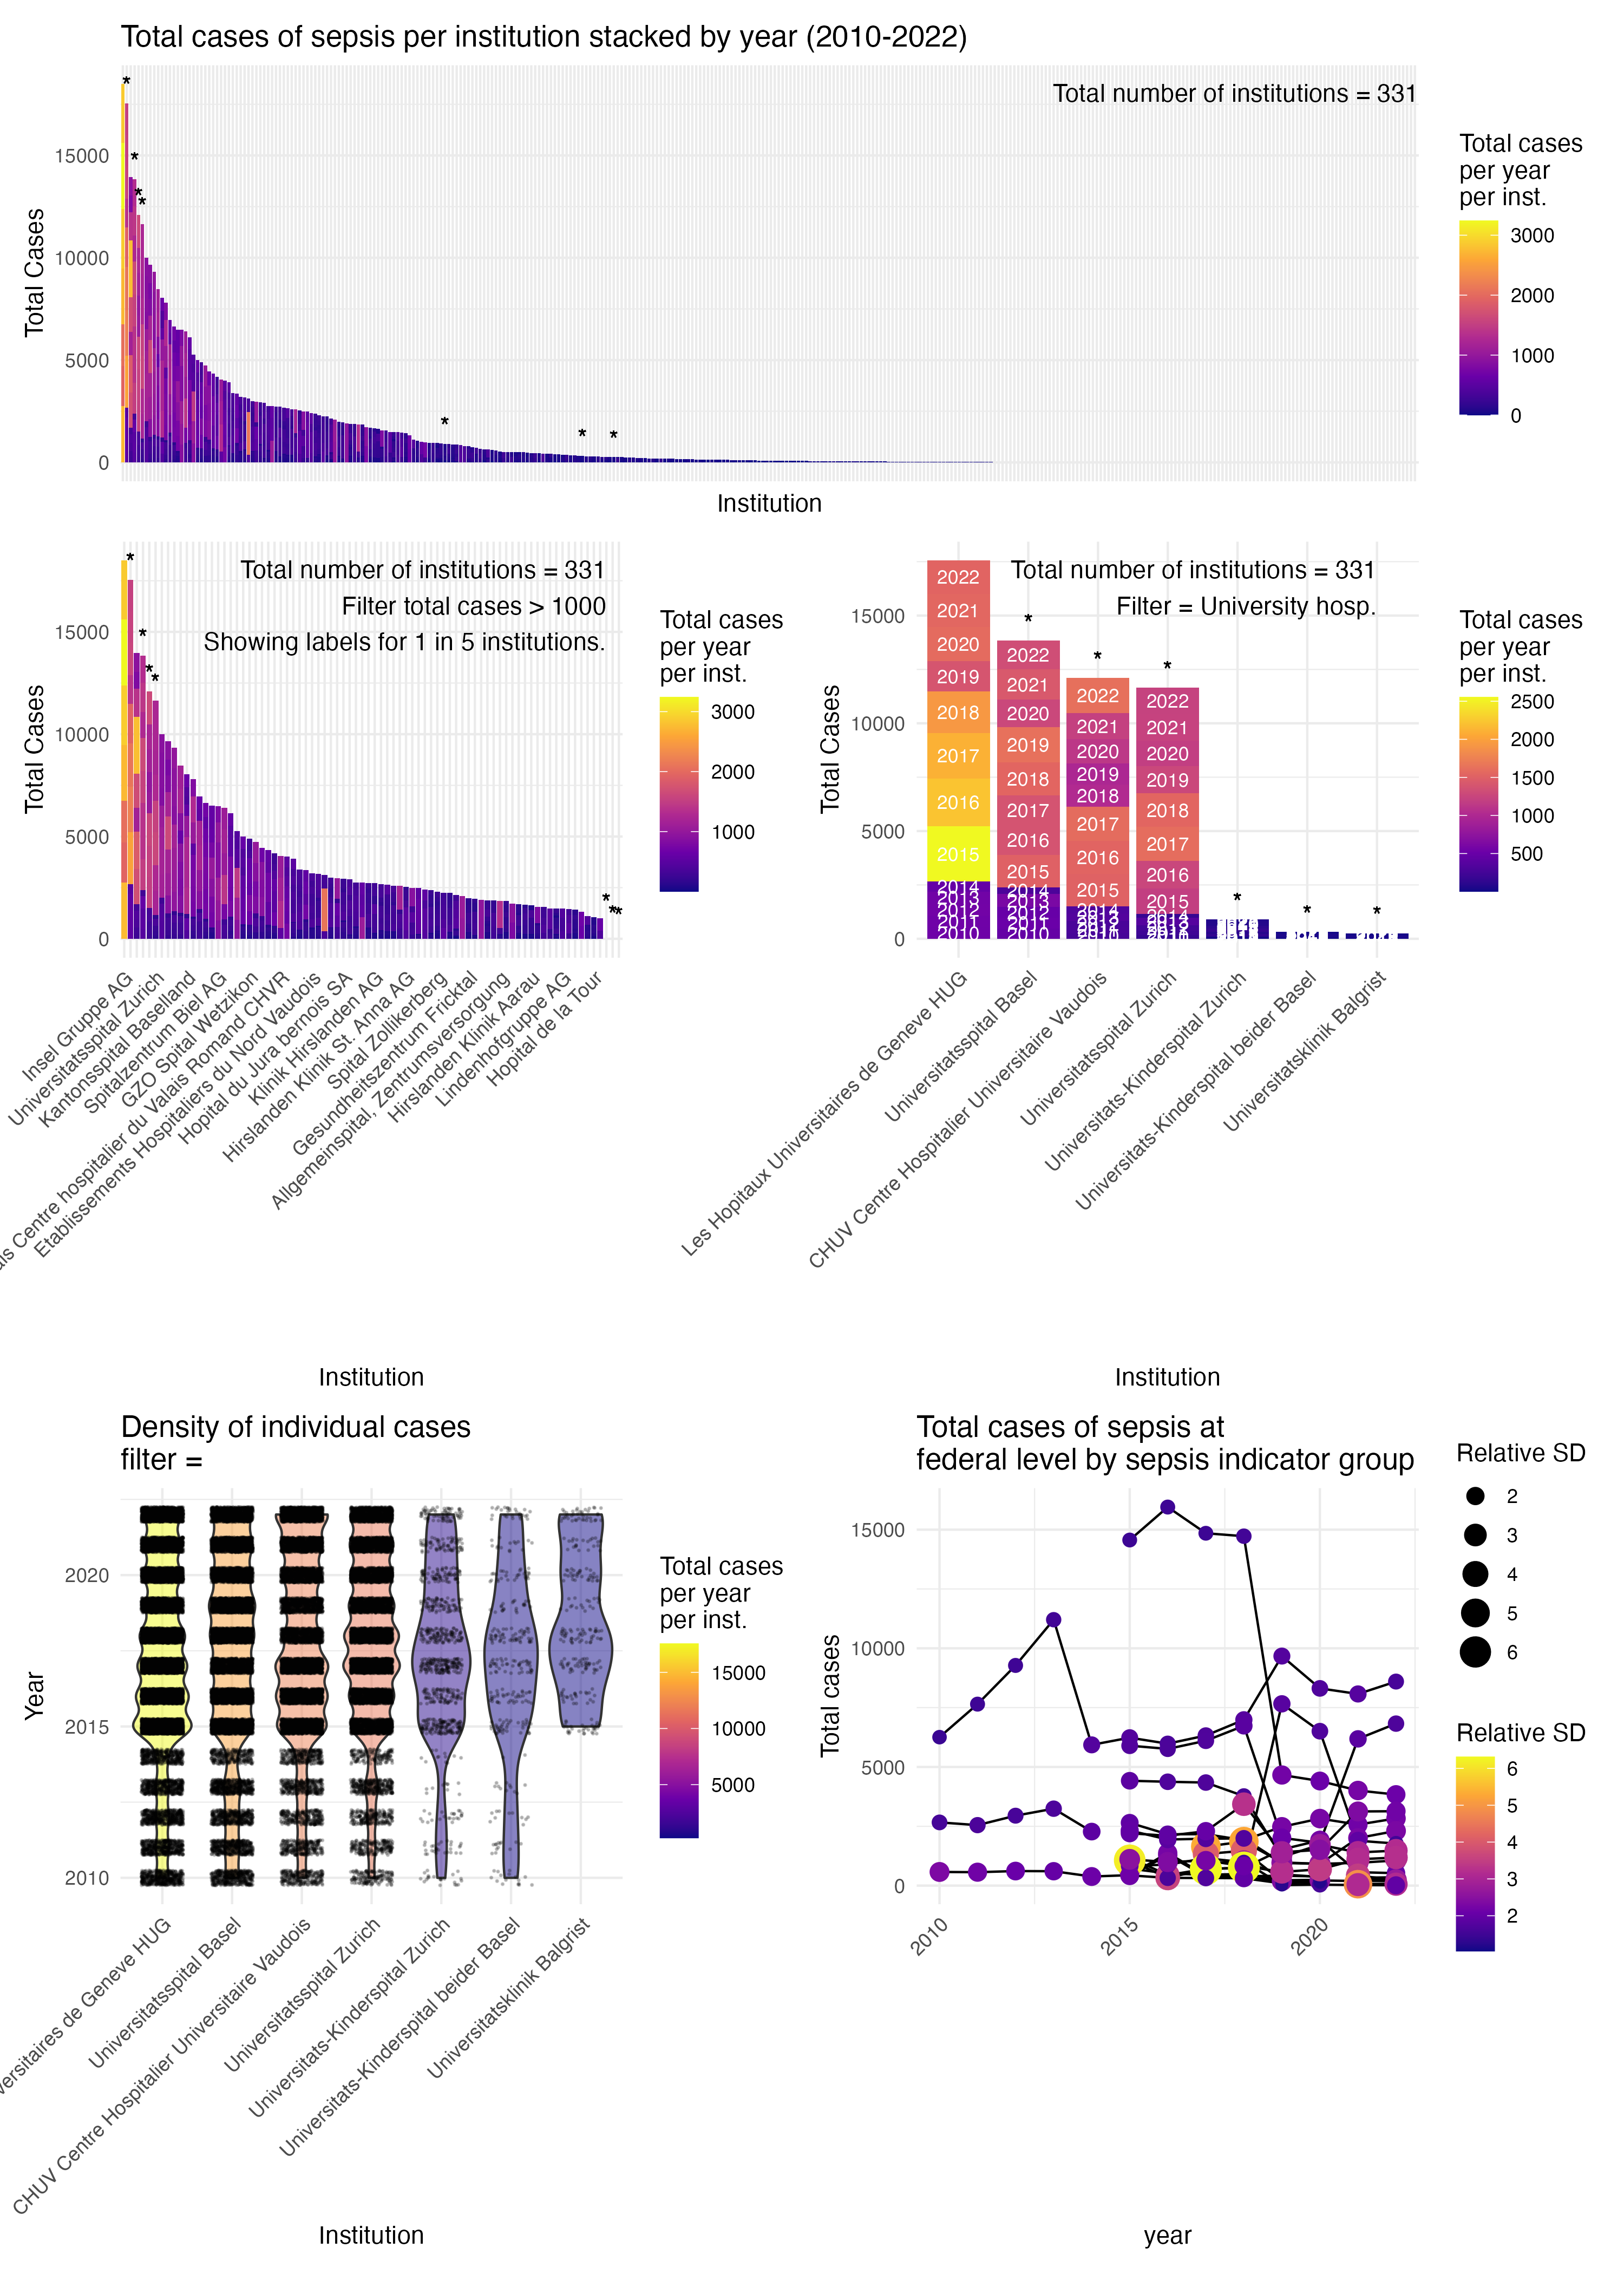
\includegraphics[width=0.90\textwidth]{../stats/foph_key_stats/output/p_patch_year_case_inst_variability_main}
	\caption{Cases per year for a national registry (detailed). Federal level number of sepsis cases from 2010-2022. These number demonstrate the number of observations required for a national registry. Federal statistics from Bundesamt für Gesundheit (BAG, Federal office for public health).}
	\label{fig:national_registry2}
\end{center}
\end{figure}

\begin{figure}[h] \hspace*{0cm} 
\begin{center}
	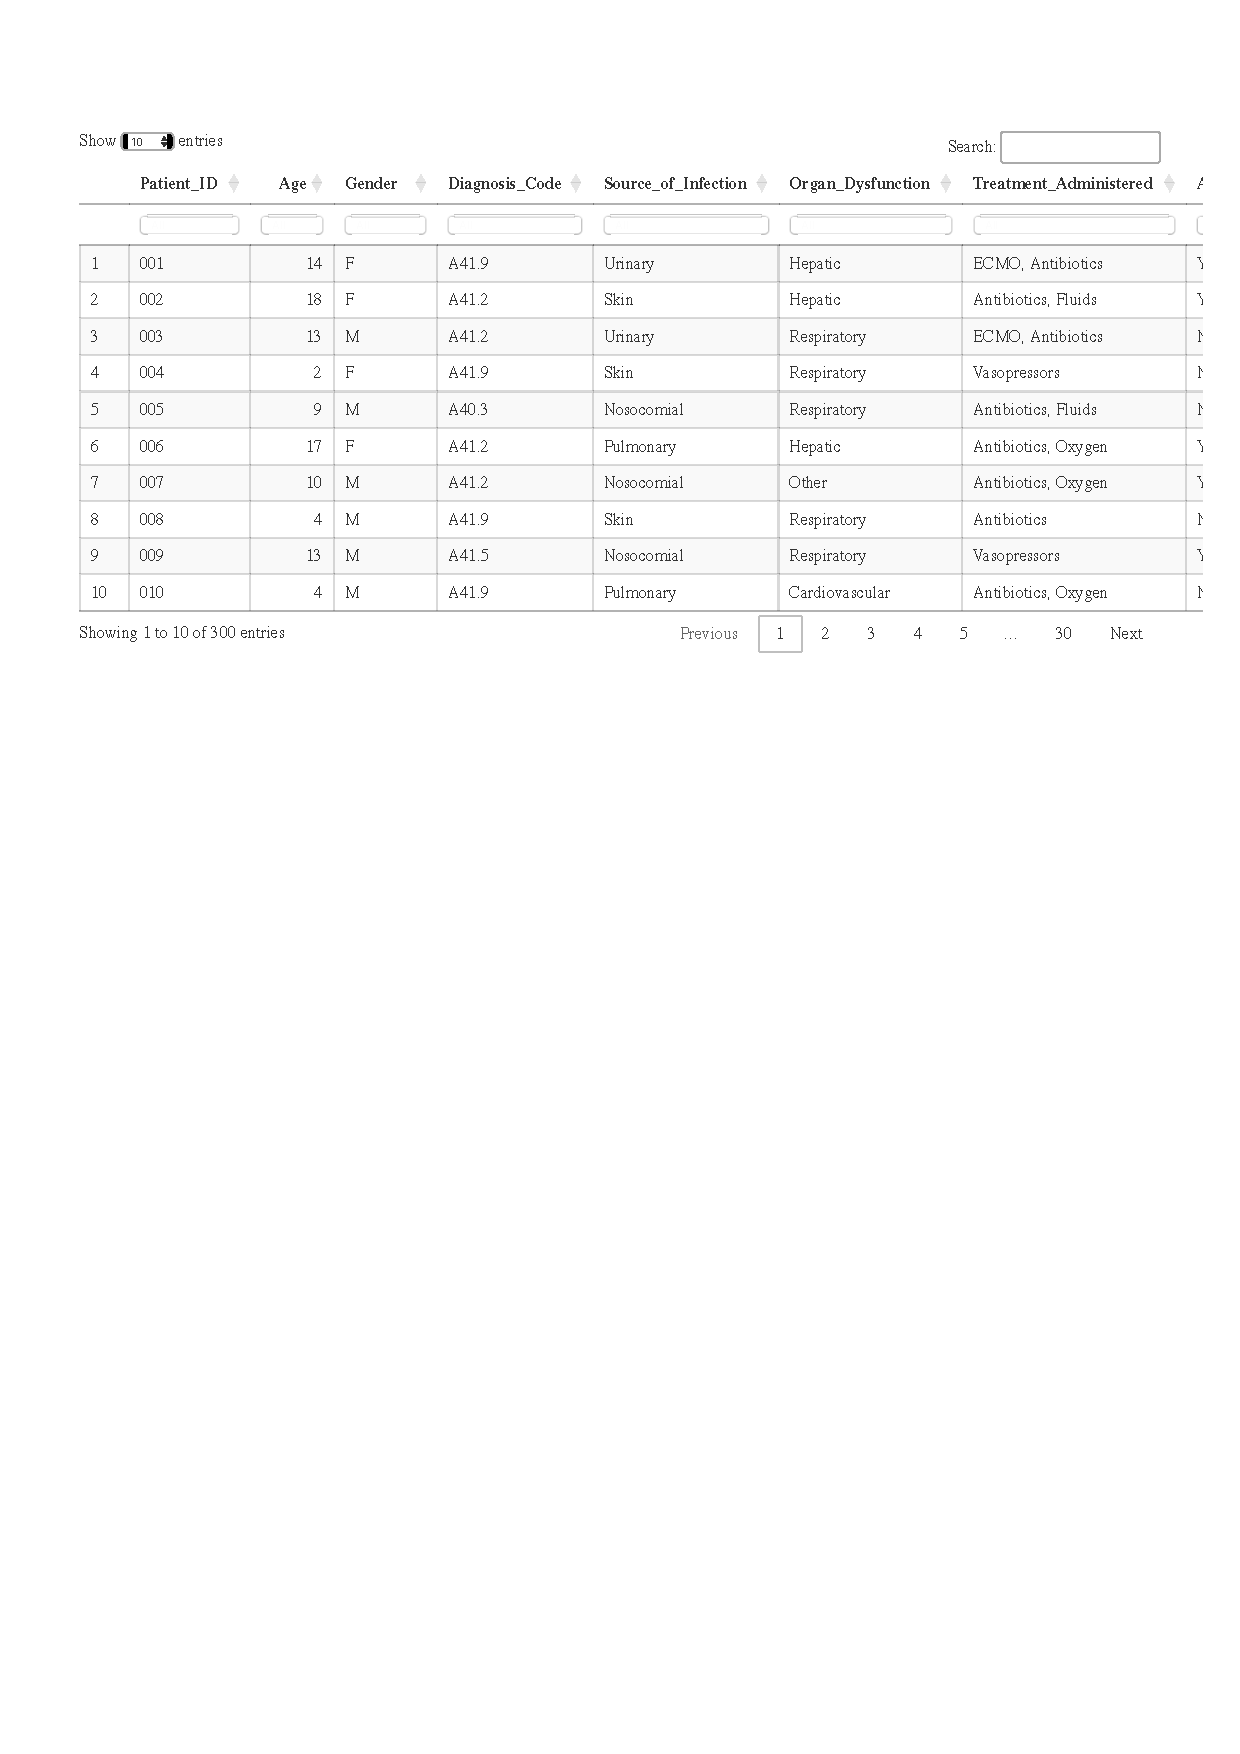
\includegraphics[width=1\textwidth]{../national_registry/data/registry_snapshot.pdf}
	\caption{Demo of a national sepsis registry made with synthetic values based on real-world samples.}
	\label{fig:national_registry_snapshot}
\end{center}
\end{figure}

Figure 
\ref{fig:national_registry_snapshot} shows a snapshot of the demo national sepsis registry.
We have included variables that cover the minimal set of features and provide a number of optional advanced features which are important to research and future development. 
Table 
\ref{tab:national_registry_example} 
shows an example of features and data types that are captured.
The current modelled variables contain:
\texttt{Patient\_ID, Age, Gender, Diagnosis\_Code, Source\_of\_Infection, Organ\_Dysfunction, Treatment\_Administered, AMS\_Compliance, National\_Sepsis\_Pathway\_Used, Outcome, Sepsis\_Standard\_Met, Date\_Admission, Date\_Discharge, Date\_Follow\_up, study\_site, sex, age\_at\_bc\_days, age\_grp, ethnicity, category, ccc\_final, hosp\_sepsis, hosp\_delay, hosp\_los, hosp\_los\_bc, pathogen\_grp, focus\_grp, picu, picu\_reason, picu\_los, picu\_los\_bc, cahai, death\_30\_bc, death\_delay, cons05\_score\_agg, pelod\_score\_agg, psofa\_score\_agg, podium\_score\_agg}.

\begin{table}[h]
        \caption{Example subset of registry data fields} 
    \centering
    \begin{tabular}{|l|>{\raggedright\arraybackslash}p{3cm}|>{\raggedright\arraybackslash}p{6cm}|}
        \hline
        \textbf{Field Name} & \textbf{Data Type} & \textbf{Description} \\
        \hline
        Patient\_ID & String & A unique identifier for each patient to ensure privacy and enable tracking. \\
        \hline
        Age & Integer & Age of the patient at the time of admission. \\
        \hline
        Gender & Char(1) & Gender of the patient (M for male, F for female). \\
        \hline
        Admission\_Date & Date & Date when the patient was admitted to the hospital. \\
        \hline
        Discharge\_Date & Date & Date when the patient was discharged from the hospital. \\
        \hline
        Diagnosis\_Code & ICD-10 Code & ICD-10 code for sepsis (e.g., A41.9 for sepsis, unspecified organisms). \\
        \hline
        Source\_of\_Infection & String & The likely source or site of the infection leading to sepsis. \\
        \hline
        Organ\_Dysfunction & Enum("Renal", "Cardiovascular", "Respiratory", "Hepatic", "Multiorgan", "Other") & Specific organs affected by sepsis. \\
        \hline
        Treatment\_Administered & Text & Key treatments provided to the patient (e.g., antibiotics, vasopressors, supportive care). \\
        \hline
        AMS\_Compliance & Boolean & Indicates whether antimicrobial stewardship (AMS) guidelines were followed (Yes/No). \\
        \hline
        National\_Sepsis\_Pathway\_Used & Boolean & Indicates if a national sepsis pathway was followed for treatment (Yes/No). \\
        \hline
        Outcome & Enum("Survived", "Deceased") & Patient's condition at discharge. \\
        \hline
        Follow\_up\_Date & Date & Date for a follow-up visit or assessment, if applicable. \\
        \hline
        Sepsis\_Standard\_Met & Boolean & Indicates whether the minimal national sepsis standard for care was met (Yes/No). \\
        \hline
    \end{tabular}
    \label{tab:national_registry_example}
 
\end{table}




